\chapter{RMS Limiter}

The limiter algorithm is implemented using an Assembler routine. From \ref{cha:CompressorDesign} is was determined that a sample size of 16 samples were needed in order to detect every frequency in the specific band, while the 0 Hz to 530 Hz needs 128 samples. In order to save calculation, the algorithm will be implemented as a running mean. Meaning a the oldest sample will be subtracted and the newest value will be added. The concept is graphically shown on \autoref{fig:RMSCompressorBlockImplmentation} where a sample is loaded and added to the sum, followed by the oldest sample being subtracted.


\begin{figure}[H]
    \centering
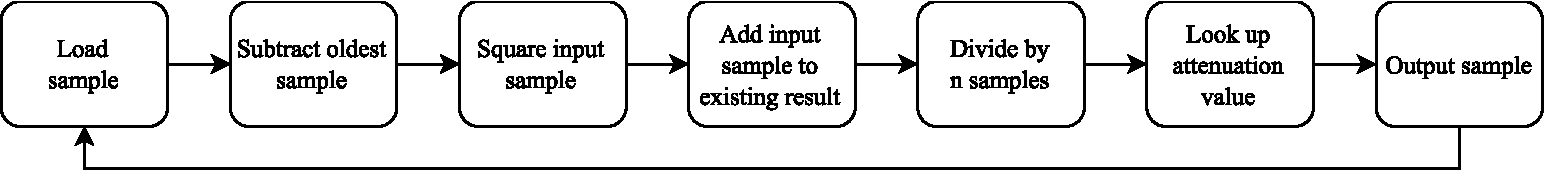
\includegraphics[width=\textwidth]{Compressor}
    \caption{Block diagram of the limiter algorithm}
    \label{fig:RMSCompressorBlockImplmentation}
\end{figure}

As mentioned the algorithm is written in Assembler by the use of a circular buffer for the samples used in the mean. %This size will determine indirectly determine the attack and release time. Both will increase simultaneously when enlarged in sample size. 
An RMS value is calculated as stated in \autoref{eq:RMScalculation}. This equation can become expensive in instruction time due to both a division and square root. These are both calculated iteratively in a processor and hence the computation time is determined by the wanted precision. \todo{kilde}

\begin{equation}\label{eq:RMScalculation}
\text{RMS}=\sqrt{\frac{1}{n}\cdot(x_1^2+x_2^2+\cdots+x_n^2)}
\end{equation}

When implemented the sample size is a value of $2^n$ which means it is then possible to bit shift the value n times to create the division. This reduces the instructions drastically. In order to handle the square root term in the expression, the value calculated will be squared. This eliminates the need for the square root term. The expression is now reduced to addition and multiplication. This is shown in equation \ref{eq:RMScalculationUSED}.

\begin{equation}\label{eq:RMScalculationUSED}
RMS^2=(\frac{1}{n}\cdot(x_1^2+x_2^2+\cdots+x_n^2))^2
\end{equation}

The algorithm will therefore be using a lookup table to determined the correct gain when the RMS$^2$ is calculated. The RMS$^2$ values of the lookup table will hence need to be quantized in order to reduce the amount of memory cells used. The steps are not to be hearable so it is determined to use steps of 0.01 since it is subjectively seen as below the audible threshold when changing gain level. The RMS$^2$ value will be changing linearly hence the lookup table values needs to be as well. The table is constructed by the use of \autoref{eq:Threslookup}. The equation calculates the needed attenuation when the threshold is exceeded and does so with a predefined step resolution. 
\vspace{-2mm}
\begin{equation}\label{eq:Threslookup}
\text{Gain}=\frac{\text{Treshold}}{\text{Threshold}+((n-1) \cdot \text{Resolution}}\enhed{.}
\end{equation}
\begin{where}
\va{$n$}{is the index number in the lookup table going from 0 to 1024}{.}
\end{where}

\vspace{2mm}
When the equation has calculated for 1024 values, the are stored in a array and converted to Q15 written in hexadecimals for implementation into the DSP.
The script for creating the values are located on a MATLAB script at: \\
\path{CD://CD/Something Somethin} \todo{PATH}

In the following listing \ref{listingCompressorMain} is a snippet of the entire RMS algorithm. Each line is commented for better overview.

\begin{lstlisting}[language={[x86masm]Assembler}, caption = {limiter Algorithm},label={listingCompressorMain}]
_RMSband
	; "Circular" data in Buffer
	MOV #dataIn4,AC0				; Load address of input data into AC0
	ADD *(#ptrBuff4),AC0			; Add the addr with the value of the data pointer (Point 					 	       to the oldest data)
	MOV AC0,AR0						; Move the addr to AR0
	MOV *AR0, AC0					; Move the value which AR0 points to into AC0
	MOV #0, AC1						; Reset AC1
	MOV uns(*(#sumLow4)), AC1       ; Move unsigned LSB of sum into AC1
	MOV uns(*(#sumHigh4))<<#16, AC2 ; Move unsigned MSB of sum into AC2
	ADD AC2, AC1					; Add AC2 to AC1 and save in AC1
	SUB AC0, AC1					; Subtract AC0/Sample from AC1/Sum and save it in AC1	 
	MOV T0, HI(AC2)					; Move the value in T0 to the high part of AC2
	MPY T0, AC2, AC2				; Square AC0 and save it in AC2
	SFTL AC2, #-15					; Bitshift the value in AC2 15 times left 
	ADD AC2, AC1					; Add AC2 to AC1 and store in AC1
	MOV AC1, *(#sumLow4)			; Move LSB in AC1 to sumLow4
	MOV HI(AC1), *(#sumHigh4)		; Move MSB in AC1 to sumHigh4
	MOV AC2, *AR0					; Move AC1 to the addr which AR0 points to
	ADD #1,*(#ptrBuff4)				; Increment the data pointer
	CMP *(#ptrBuff4)==#16,TC1		; Check if the data pointer should reset to 0
	CALLCC resetptrBuff4, TC1		; If data pointer should be reset, call reset routine
	SFTL AC1, #-9					; Divide by X to get mean
	MOV AC1,*(#RMS3)				; Save value for GUI output
	ADD #lookUpBand4, AC1			; Adjust the value to correct loaction in memory
	MOV AC1, AR0					; Move gain value addr into AR0
	MOV *AR0, AC0					; Move gain value into AC0
	SFTL AC0, #16					; Shift AC0 16 times to put as MSB in AC0
	MPY T0, AC0, AC1				; Multiply AC0 with AC1 and store in AC1 
	SFTL AC1, #-15					; Shift AC1 by 15 to create a 16 bit value
	MOV AC1, T0						; Move AC1 to T0 for function return
	RET								; Return
\end{lstlisting}

Where: \\
- dataIn4, contains the input sample from the buffer. \\
- ptrBuff4, is the circular buffer pointer. \\
- lookUpBand4, is start address for the lookup table\\
- sumHigh4, is a 16-bit value for storing MSB \\
- sumLow4, is a 16-bit value for storing LSB \\
- RMS3, is an address used for GUI output \\

\subsubsection*{Flow}


The algorithm starts by subtracting the oldest 16-bit sample from the sum. Then the new 16-bit sample in T0 is squared and added. The 32-bit value is saved in sumHigh and sumLow. The pointer which keeps track of the samples is then incremented and checked if has reached 16 samples. If 16 samples has been calculated it will reset.

The MSB of the sum is then used to locate the desired gain value in the look up table. The value calculated will act as an offset to the start address in the lookup table. Meaning if the input is so low it yields 0, it will take the first value in the table which is 1. Should the input be high enough to produce a number it will use that number as an offset to determine the prober address. This means that when the value is to be divided it should be shifted 4 times due to the amount of samples. Next it should shifted 5 times before added to the lookup tables start value. The reason of the last 5 shifts is due to the size of the lookup table, which is of 128 values. This corresponds with 7 bits. This removes the chance of overflow, since the possible maximum value will now take the 128'th place in the table. The complete Look up table can be found at \autoref{app:LookupTables}. 

When the value has been determined it is multiplied with the MSB of sum. This yields again a 32-bit where the MSB is stored in T0, which is used as output of the function.


\section{Release time}

If no release time is implied to the limiter the compression will be too aggressive, which will result in a distorted sound. The release time is basically the time span for the limiter to release the gain reduction. Implementing a release time also ensures that the compression is not constantly switch between two different gains. The release time will be implemented as a first order IIR filter where the release time will be the time constant $\tau$. The general design and implementation procedure for IIR filters are described in \autoref{ch:IIR}. The release time is chosen to be 5 seconds, as 5 seconds is estimated to be sufficient.

It is commonly known that an analog first order filter can be designed as following expression:
\begin{equation}
H(s) = \frac{\omega_c}{s+\omega_c}
\end{equation}
As $\tau = 5\, s$ and the natural frequency is $\omega_c = \frac{1}{\tau}$ then the transfer function for the first order filter is:
\begin{equation}
H(s) = \frac{0.2}{s+0.2}
\end{equation} 
A pole is located at -0.2 and the cutoff frequency can be calculated as $f = \frac{0.2}{2\pi} = 0.0318 \text{Hz}$. The frequency response of the transfer function and the step response of the filter are now plotted to examine if the filter has the desired response:

\begin{figure}[H]
\centering
\begin{subfigure}[t]{0.7\textwidth}
	\tikzsetnextfilename{releaseTimeAnalogFreq}
	% This file was created by matlab2tikz.
%
%The latest updates can be retrieved from
%  http://www.mathworks.com/matlabcentral/fileexchange/22022-matlab2tikz-matlab2tikz
%where you can also make suggestions and rate matlab2tikz.
%
\definecolor{mycolor1}{rgb}{0.00000,0.44700,0.74100}%
%
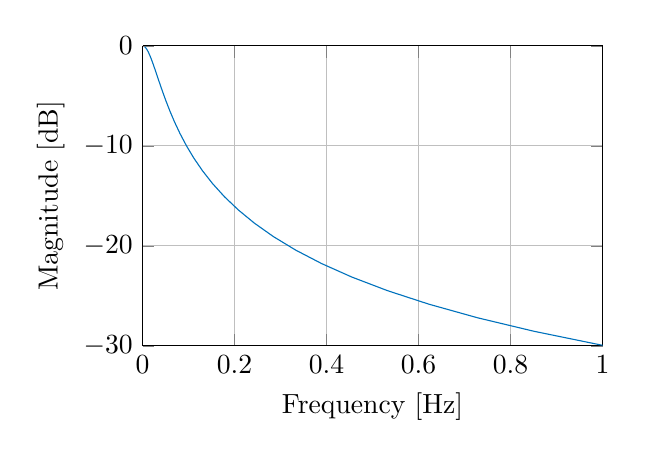
\begin{tikzpicture}

\begin{axis}[%
width=2.3in,
height=1.5in,
at={(1.178in,0.642in)},
scale only axis,
separate axis lines,
every outer x axis line/.append style={black},
every x tick label/.append style={font=\color{black}},
xmin=0,
xmax=1,
xlabel={Frequency [Hz]},
xmajorgrids,
every outer y axis line/.append style={black},
every y tick label/.append style={font=\color{black}},
ymin=-30,
ymax=0,
ylabel={Magnitude [dB]},
ymajorgrids,
axis background/.style={fill=white}
]
\addplot [color=mycolor1,solid,forget plot]
  table[row sep=crcr]{%
0.00486793224963312	-0.100402222082808\\
0.00569250375018921	-0.136721464088196\\
0.00665674813949196	-0.185900319494538\\
0.00778432439173304	-0.252261956056567\\
0.00910289903808118	-0.341398619864277\\
0.0106448250005485	-0.460402462824248\\
0.0124479354124735	-0.618031667021366\\
0.014556471903026	-0.824722461824115\\
0.017022170122385	-1.09232865997336\\
0.0199055291423454	-1.43346931758523\\
0.0232772958787259	-1.86042522209172\\
0.027220200957788	-2.3836676448467\\
0.0318309886183791	-3.01029995663981\\
0.0372227904560523	-3.74284364831552\\
0.0435279012520263	-4.57877722902935\\
0.0509010249955101	-5.51099732799167\\
0.0595230707447199	-6.52903267384862\\
0.0696055914629116	-7.62060247916819\\
0.0813959747419707	-8.77308768783426\\
0.0951835127746273	-9.97463448710595\\
0.111306500509859	-11.2148066476148\\
0.130160536153839	-12.4848459872759\\
0.152208227679875	-13.7776603541827\\
0.177990543509032	-15.0876575022452\\
0.208140085864946	-16.4105142637086\\
0.243396612481656	-17.7429372129771\\
0.28462518750946	-19.0824444476297\\
0.332837406974598	-20.4271805179842\\
0.389216219586652	-21.7757664430774\\
0.455144951904059	-23.12718177754\\
0.532241250027424	-24.4806737842602\\
0.622396770623676	-25.8356884927786\\
0.727823595151299	-27.1918189075576\\
0.851108506119248	-28.5487663867961\\
0.99527645711727	-29.9063119957401\\
1.16386479393629	-31.2642953402859\\
};
\end{axis}
\end{tikzpicture}%
	\caption{Frequency response.}
	\label{fig:releaseTimeAnalogFreq}
\end{subfigure}
\begin{subfigure}[t]{0.7\textwidth}
	\tikzsetnextfilename{releaseTimeAnalogStep}
	% This file was created by matlab2tikz.
%
%The latest updates can be retrieved from
%  http://www.mathworks.com/matlabcentral/fileexchange/22022-matlab2tikz-matlab2tikz
%where you can also make suggestions and rate matlab2tikz.
%
\definecolor{mycolor1}{rgb}{0.00000,0.44700,0.74100}%
%
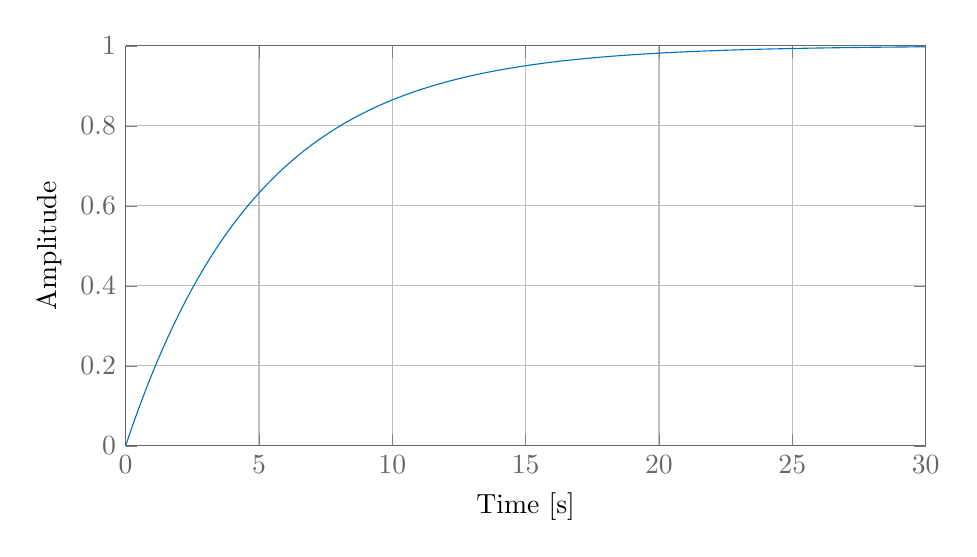
\begin{tikzpicture}

\begin{axis}[%
width=4in,
height=2in,
at={(1.178in,0.642in)},
scale only axis,
separate axis lines,
every outer x axis line/.append style={white!40!black},
every x tick label/.append style={font=\color{white!40!black}},
xmin=0,
xmax=30,
xlabel={Time [s]},
xmajorgrids,
every outer y axis line/.append style={white!40!black},
every y tick label/.append style={font=\color{white!40!black}},
ymin=0,
ymax=1,
ylabel={Amplitude},
ymajorgrids,
axis background/.style={fill=white}
]
\addplot [color=mycolor1,solid,forget plot]
  table[row sep=crcr]{%
0	0\\
0.230258509299149	0.0450074139785152\\
0.460517018598298	0.087989160643997\\
0.690775527897447	0.129036410043786\\
0.921034037196596	0.168236228897159\\
1.15129254649574	0.205671765275515\\
1.38155105579489	0.241422424970584\\
1.61180956509404	0.275564039924751\\
1.84206807439319	0.308169029080781\\
2.07232658369234	0.3393065519921\\
2.30258509299149	0.369042655519484\\
2.53284360229064	0.397440413925303\\
2.76310211158979	0.42456006266249\\
2.99336062088894	0.45045912614201\\
3.22361913018809	0.475192539749852\\
3.45387763948723	0.498812766372343\\
3.68413614878638	0.52136990767697\\
3.91439465808553	0.542911810384727\\
4.14465316738468	0.563484167759432\\
4.37491167668383	0.583130616529259\\
4.60517018598298	0.601892829446095\\
4.83542869528213	0.61981060367903\\
5.06568720458128	0.63692194522949\\
5.29594571388043	0.65326314954706\\
5.52620422317958	0.668868878517002\\
5.75646273247872	0.683772233982758\\
5.98672124177787	0.698004827959397\\
6.21697975107702	0.711596849686941\\
6.44723826037617	0.724577129665789\\
6.67749676967532	0.736973200810072\\
6.90775527897447	0.748811356848656\\
7.13801378827362	0.76011670809767\\
7.36827229757277	0.770913234722848\\
7.59853080687192	0.781223837604675\\
7.82878931617106	0.791070386914232\\
8.05904782547021	0.800473768502755\\
8.28930633476936	0.809453928203324\\
8.51956484406851	0.818029914138657\\
8.74982335336766	0.826219917124725\\
8.98008186266681	0.834041309255913\\
9.21034037196596	0.841510680753564\\
9.44059888126511	0.848643875156062\\
9.67085739056426	0.855456022925097\\
9.90111589986341	0.861961573539408\\
10.1313744091626	0.868174326144063\\
10.3616329184617	0.874107458820294\\
10.5918914277609	0.879773556537976\\
10.82214993706	0.885184637850036\\
11.0524084463592	0.890352180385413\\
11.2826669556583	0.895287145194648\\
11.5129254649574	0.899999999999745\\
11.7431839742566	0.904500741397608\\
11.9734424835557	0.908798916064167\\
12.2037009928549	0.912903641004156\\
12.433959502154	0.916823622889504\\
12.6642180114532	0.920567176527349\\
12.8944765207523	0.924142242496865\\
13.1247350300515	0.927556403992291\\
13.3549935393506	0.930816902907902\\
13.5852520486498	0.933930655199042\\
13.8155105579489	0.936904265551788\\
14.0457690672481	0.939744041392377\\
14.2760275765472	0.942456006266103\\
14.5062860858464	0.945045912614061\\
14.7365445951455	0.947519253974852\\
14.9668031044447	0.949881276637107\\
15.1970616137438	0.952136990767576\\
15.427320123043	0.954291181038357\\
15.6575786323421	0.956348416775833\\
15.8878371416413	0.95831306165282\\
16.1180956509404	0.960189282944509\\
16.3483541602396	0.961981060367807\\
16.5786126695387	0.963692194522857\\
16.8088711788379	0.965326314954619\\
17.039129688137	0.966886887851617\\
17.2693881974362	0.968377223398196\\
17.4996467067353	0.969800482795864\\
17.7299052160345	0.971159684968621\\
17.9601637253336	0.97245771296651\\
18.1904222346328	0.973697320080941\\
18.4206807439319	0.974881135684803\\
18.6509392532311	0.976011670809707\\
18.8811977625302	0.977091323472227\\
19.1114562718294	0.978122383760413\\
19.3417147811285	0.979107038691371\\
19.5719732904277	0.980047376850226\\
19.8022317997268	0.980945392820285\\
20.032490309026	0.98180299141382\\
20.2627488183251	0.982621991712429\\
20.4930073276243	0.98340413092555\\
20.7232658369234	0.984151068075317\\
20.9535243462226	0.984864387515568\\
21.1837828555217	0.985545602292474\\
21.4140413648209	0.986196157353906\\
21.64429987412	0.986817432614373\\
21.8745583834191	0.987410745881998\\
22.1048168927183	0.987977355653768\\
22.3350754020174	0.988518463784975\\
22.5653339113166	0.989035218038514\\
22.7955924206157	0.989528714519439\\
23.0258509299149	0.98999999999995\\
23.256109439214	0.990450074139737\\
23.4863679485132	0.990879891606394\\
23.7166264578123	0.991290364100394\\
23.9468849671115	0.99168236228893\\
24.1771434764106	0.992056717652715\\
24.4074019857098	0.992414224249668\\
24.6376604950089	0.992755640399211\\
24.8679190043081	0.993081690290773\\
25.0981775136072	0.993393065519888\\
25.3284360229064	0.993690426555163\\
25.5586945322055	0.993974404139223\\
25.7889530415047	0.994245600626596\\
26.0192115508038	0.994504591261393\\
26.249470060103	0.994751925397473\\
26.4797285694021	0.994988127663699\\
26.7099870787013	0.995213699076746\\
26.9402455880004	0.995429118103825\\
27.1705040972996	0.995634841677573\\
27.4007626065987	0.995831306165272\\
27.6310211158979	0.996018928294442\\
27.861279625197	0.996198106036772\\
28.0915381344962	0.996369219452278\\
28.3217966437953	0.996532631495454\\
28.5520551530945	0.996688688785154\\
28.7823136623936	0.996837722339813\\
29.0125721716928	0.99698004827958\\
29.2428306809919	0.997115968496856\\
29.4730891902911	0.997245771296645\\
29.7033476995902	0.997369732008088\\
29.9336062088894	0.997488113568475\\
30.1638647181885	0.997601167080966\\
30.3941232274877	0.997709132347218\\
30.6243817367868	0.997812238376037\\
30.854640246086	0.997910703869133\\
31.0848987553851	0.998004737685019\\
31.3151572646843	0.998094539282025\\
31.5454157739834	0.998180299141379\\
31.7756742832826	0.99826219917124\\
32.0059327925817	0.998340413092552\\
32.2361913018809	0.998415106807529\\
32.46644981118	0.998486438751554\\
32.6967083204792	0.998554560229245\\
32.9269668297783	0.998619615735388\\
33.1572253390774	0.998681743261435\\
33.3874838483766	0.998741074588198\\
33.6177423576757	0.998797735565375\\
33.8480008669749	0.998851846378496\\
34.078259376274	0.99890352180385\\
34.3085178855732	0.998952871451942\\
34.5387763948723	0.998999999999993\\
34.7690349041715	0.999045007413972\\
34.9992934134706	0.999087989160638\\
35.2295519227698	0.999129036410038\\
35.4598104320689	0.999168236228892\\
35.6900689413681	0.999205671765271\\
35.9203274506672	0.999241422424966\\
36.1505859599664	0.99927556403992\\
36.3808444692655	0.999308169029077\\
36.6111029785647	0.999339306551988\\
36.8413614878638	0.999369042655516\\
37.071619997163	0.999397440413922\\
37.3018785064621	0.999424560062659\\
37.5321370157613	0.999450459126139\\
37.7623955250604	0.999475192539747\\
37.9926540343596	0.99949881276637\\
38.2229125436587	0.999521369907674\\
38.4531710529579	0.999542911810382\\
38.683429562257	0.999563484167757\\
38.9136880715562	0.999583130616527\\
39.1439465808553	0.999601892829444\\
39.3742050901545	0.999619810603677\\
39.6044635994536	0.999636921945228\\
39.8347221087528	0.999653263149546\\
40.0649806180519	0.999668868878516\\
40.2952391273511	0.999683772233981\\
40.5254976366502	0.999698004827958\\
40.7557561459494	0.999711596849686\\
40.9860146552485	0.999724577129665\\
41.2162731645477	0.999736973200809\\
41.4465316738468	0.999748811356848\\
41.676790183146	0.999760116708097\\
41.9070486924451	0.999770913234722\\
42.1373072017443	0.999781223837604\\
42.3675657110434	0.999791070386914\\
42.5978242203426	0.999800473768502\\
42.8280827296417	0.999809453928203\\
43.0583412389409	0.999818029914138\\
43.28859974824	0.999826219917125\\
43.5188582575392	0.999834041309256\\
43.7491167668383	0.999841510680754\\
43.9793752761375	0.999848643875156\\
44.2096337854366	0.999855456022925\\
44.4398922947357	0.99986196157354\\
44.6701508040349	0.999868174326144\\
44.900409313334	0.999874107458821\\
45.1306678226332	0.999879773556538\\
45.3609263319323	0.99988518463785\\
45.5911848412315	0.999890352180386\\
45.8214433505306	0.999895287145195\\
46.0517018598298	0.9999\\
46.2819603691289	0.999904500741398\\
46.5122188784281	0.999908798916065\\
46.7424773877272	0.999912903641005\\
46.9727358970264	0.99991682362289\\
47.2029944063255	0.999920567176528\\
47.4332529156247	0.999924142242497\\
47.6635114249238	0.999927556403993\\
47.893769934223	0.999930816902909\\
48.1240284435221	0.9999339306552\\
48.3542869528213	0.999936904265553\\
48.5845454621204	0.999939744041393\\
48.8148039714196	0.999942456006267\\
49.0450624807187	0.999945045912615\\
49.2753209900179	0.999947519253976\\
49.505579499317	0.999949881276638\\
49.7358380086162	0.999952136990769\\
49.9660965179153	0.99995429118104\\
50.1963550272145	0.999956348416777\\
50.4266135365136	0.999958313061654\\
50.6568720458128	0.999960189282946\\
50.8871305551119	0.999961981060369\\
51.1173890644111	0.999963692194524\\
51.3476475737102	0.999965326314956\\
51.5779060830094	0.999966886887853\\
51.8081645923085	0.999968377223399\\
52.0384231016077	0.999969800482797\\
52.2686816109068	0.99997115968497\\
52.498940120206	0.999972457712967\\
52.7291986295051	0.999973697320082\\
};
\end{axis}
\end{tikzpicture}%
	\caption{Step response.}
	\label{fig:releaseTimeAnalogStep}
\end{subfigure}
\caption{The frequency response and step response of the analog filter.}
\label{fig:releaseTimeAnalog}
\end{figure}

It is seen that the -3 dB cutoff frequency is located at 0,0318 Hz in \autoref{fig:releaseTimeAnalogFreq} and the release time is 5 seconds as the 66\% rise time is located at 5 seconds. To implement the filter on a DSP, the transfer function is now transformed into z-domain. The chosen transformation is the impulse invariant. An explanation of the impulse invariant and bilinear transformation is provided in \autoref{ch:IIR}. By using the impulse invariant method following transfer function is obtained.
\begin{equation} \label{eq:releaseTF}
H(z) = T\frac{0.2}{1-\text{e}^{-0.2T} z^{-1}}
\end{equation} 
The Sampling period, T, varies as it depends on which octave band it is implemented into. In the following example, the sampling period is $T = 2.667$ ms or $f_s = 375$ which corresponds to the sampling rate for the lowest octave band. The filter coefficient is obtained to quantized them in order to examine if the frequency response and step response of the filter still has the desired characteristic when implementing the filter in DSP. To apply quantization, the coefficients are first multiplied with $2^{15}$ (Q15 format) and then rounded. Afterwards the coefficients are divided by $2^{15}$ to obtain a floating point number. After the quantization, the frequency response and step response is now plotted to examine the filter.

\begin{figure}[H]
\centering
\begin{subfigure}[t]{0.7\textwidth}
	\tikzsetnextfilename{releaseTimeDigitalFreq}
	% This file was created by matlab2tikz.
%
%The latest updates can be retrieved from
%  http://www.mathworks.com/matlabcentral/fileexchange/22022-matlab2tikz-matlab2tikz
%where you can also make suggestions and rate matlab2tikz.
%
\definecolor{mycolor1}{rgb}{0.00000,0.44700,0.74100}%
%
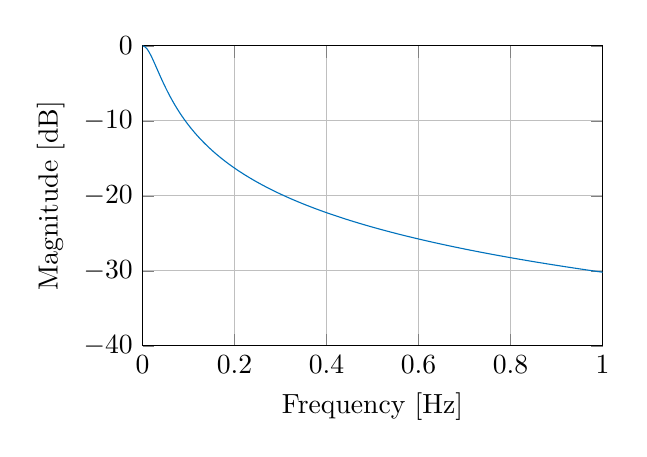
\begin{tikzpicture}

\begin{axis}[%
width=2.3in,
height=1.5in,
at={(1.011in,3.406in)},
scale only axis,
unbounded coords=jump,
xmin=0,
xmax=1,
xlabel={Frequency [Hz]},
xmajorgrids,
ymin=-40,
ymax=0,
ylabel={Magnitude [dB]},
ymajorgrids,
axis background/.style={fill=white}
]
\addplot [color=mycolor1,solid,forget plot]
  table[row sep=crcr]{%
0	0\\
0.005	-0.111737595123031\\
0.01	-0.43067199650568\\
0.015	-0.915126616733801\\
0.02	-1.51369200111139\\
0.025	-2.17894140857373\\
0.03	-2.87408720765069\\
0.035	-3.57373707425285\\
0.04	-4.26184436446715\\
0.045	-4.92907225693824\\
0.05	-5.57054218469563\\
0.055	-6.18419052237221\\
0.06	-6.7696604420878\\
0.065	-7.32758711398577\\
0.07	-7.85914917885435\\
0.075	-8.36579296562235\\
0.08	-8.8490661988676\\
0.085	-9.31052016626757\\
0.09	-9.75165429578954\\
0.095	-10.1738867816785\\
0.1	-10.5785410388897\\
0.105	-10.9668416203498\\
0.11	-11.339915642506\\
0.115	-11.6987972718709\\
0.12	-12.0444337682722\\
0.125	-12.3776921709963\\
0.13	-12.6993660837707\\
0.135	-13.0101822456238\\
0.14	-13.310806718433\\
0.145	-13.6018506105917\\
0.15	-13.8838753100013\\
0.155	-14.157397231362\\
0.16	-14.4228921006709\\
0.165	-14.6807988091067\\
0.17	-14.9315228724394\\
0.175	-15.175439532826\\
0.18	-15.4128965387148\\
0.185	-15.6442166364032\\
0.19	-15.8696998041316\\
0.195	-16.0896252567567\\
0.2	-16.3042532462347\\
0.205	-16.5138266804717\\
0.21	-16.7185725806136\\
0.215	-16.9187033945881\\
0.22	-17.1144181826717\\
0.225	-17.3059036890315\\
0.23	-17.4933353115754\\
0.235	-17.6768779810085\\
0.24	-17.8566869587333\\
0.245	-18.0329085621139\\
0.25	-18.2056808246487\\
0.255	-18.3751340977329\\
0.26	-18.541391599935\\
0.265	-18.7045699190468\\
0.27	-18.8647794715815\\
0.275	-19.0221249238775\\
0.28	-19.1767055785142\\
0.285	-19.3286157293434\\
0.29	-19.47794498809\\
0.295	-19.624778585161\\
0.3	-19.7691976470285\\
0.305	-19.9112794523059\\
0.31	-20.0510976684226\\
0.315	-20.1887225706086\\
0.32	-20.3242212447292\\
0.325	-20.4576577753613\\
0.33	-20.5890934203624\\
0.335	-20.7185867730677\\
0.34	-20.8461939131395\\
0.345	-20.9719685469975\\
0.35	-21.0959621386733\\
0.355	-21.2182240318525\\
0.36	-21.3388015638018\\
0.365	-21.4577401718123\\
0.37	-21.5750834927367\\
0.375	-21.6908734561454\\
0.38	-21.8051503715832\\
0.385	-21.9179530103647\\
0.39	-22.0293186823094\\
0.395	-22.1392833077871\\
0.4	-22.247881485408\\
0.405	-22.3551465556685\\
0.41	-22.4611106608381\\
0.415	-22.5658048013468\\
0.42	-22.6692588889158\\
0.425	-22.7715017966521\\
0.43	-22.8725614063114\\
0.435	-22.9724646529193\\
0.44	-23.0712375669228\\
0.445	-23.1689053140362\\
0.45	-23.2654922329272\\
0.455	-23.3610218708837\\
0.46	-23.4555170175885\\
0.465	-23.5489997371191\\
0.47	-23.6414913982848\\
0.475	-23.733012703402\\
0.48	-23.823583715603\\
0.485	-23.9132238847667\\
0.49	-24.0019520721527\\
0.495	-24.0897865738175\\
0.5	-24.1767451428812\\
0.505	-24.2628450107142\\
0.51	-24.3481029071033\\
0.515	-24.4325350794584\\
0.52	-24.5161573111103\\
0.525	-24.5989849387535\\
0.53	-24.6810328690802\\
0.535	-24.7623155946494\\
0.54	-24.8428472090332\\
0.545	-24.9226414212803\\
0.55	-25.0017115697308\\
0.555	-25.0800706352197\\
0.56	-25.1577312536985\\
0.565	-25.2347057283071\\
0.57	-25.3110060409236\\
0.575	-25.3866438632192\\
0.58	-25.4616305672427\\
0.585	-25.5359772355588\\
0.59	-25.6096946709629\\
0.595	-25.6827934057925\\
0.6	-25.7552837108554\\
0.605	-25.8271756039941\\
0.61	-25.898478858303\\
0.615	-25.9692030100154\\
0.62	-26.0393573660771\\
0.625	-26.1089510114189\\
0.63	-26.1779928159455\\
0.635	-26.2464914412509\\
0.64	-26.3144553470751\\
0.645	-26.3818927975127\\
0.65	-26.4488118669857\\
0.655	-26.5152204459903\\
0.66	-26.5811262466279\\
0.665	-26.6465368079308\\
0.67	-26.7114595009911\\
0.675	-26.7759015339005\\
0.68	-26.8398699565117\\
0.685	-26.903371665026\\
0.69	-26.9664134064172\\
0.695	-27.0290017826979\\
0.7	-27.0911432550335\\
0.705	-27.1528441477131\\
0.71	-27.2141106519807\\
0.715	-27.2749488297341\\
0.72	-27.3353646170956\\
0.725	-27.3953638278621\\
0.73	-27.454952156836\\
0.735	-27.5141351830451\\
0.74	-27.5729183728542\\
0.745	-27.6313070829726\\
0.75	-27.6893065633625\\
0.755	-27.7469219600521\\
0.76	-27.8041583178558\\
0.765	-27.861020583007\\
0.77	-27.9175136057058\\
0.775	-27.9736421425852\\
0.78	-28.0294108590978\\
0.785	-28.0848243318285\\
0.79	-28.1398870507336\\
0.795	-28.1946034213096\\
0.8	-28.2489777666956\\
0.805	-28.3030143297101\\
0.81	-28.3567172748255\\
0.815	-28.4100906900824\\
0.82	-28.463138588946\\
0.825	-28.5158649121061\\
0.83	-28.5682735292238\\
0.835	-28.6203682406261\\
0.84	-28.6721527789498\\
0.845	-28.7236308107373\\
0.85	-28.7748059379862\\
0.855	-28.825681699653\\
0.86	-28.8762615731143\\
0.865	-28.9265489755845\\
0.87	-28.9765472654947\\
0.875	-29.0262597438312\\
0.88	-29.0756896554367\\
0.885	-29.1248401902743\\
0.89	-29.1737144846571\\
0.895	-29.2223156224429\\
0.9	-29.2706466361959\\
0.905	-29.3187105083172\\
0.91	-29.366510172143\\
0.915	-29.4140485130142\\
0.92	-29.4613283693167\\
0.925	-29.5083525334931\\
0.93	-29.5551237530283\\
0.935	-29.6016447314082\\
0.94	-29.6479181290528\\
0.945	-29.6939465642256\\
0.95	-29.7397326139185\\
0.955	-29.7852788147134\\
0.96	-29.8305876636223\\
0.965	-29.875661618905\\
0.97	-29.9205031008659\\
0.975	-29.9651144926308\\
0.98	-30.0094981409035\\
0.985	-30.0536563567038\\
0.99	-30.0975914160862\\
0.995	-30.1413055608416\\
1	-30.1848009991803\\
1.005	-30.228079906399\\
1.01	-30.2711444255314\\
1.015	-30.3139966679815\\
1.02	-30.3566387141437\\
1.025	-30.3990726140056\\
1.03	-30.4413003877372\\
1.035	-30.4833240262664\\
1.04	-30.5251454918396\\
1.045	-30.56676671857\\
1.05	-30.6081896129716\\
1.055	-30.6494160544824\\
1.06	-30.6904478959734\\
1.065	-30.7312869642469\\
1.07	-30.7719350605229\\
1.075	-30.8123939609139\\
1.08	-30.8526654168891\\
1.085	-30.892751155728\\
1.09	-30.9326528809631\\
1.095	-30.9723722728132\\
1.1	-31.0119109886064\\
1.105	-31.0512706631935\\
1.11	-31.0904529093526\\
1.115	-31.1294593181846\\
};
\end{axis}
\end{tikzpicture}%
	\caption{Frequency response.}
	\label{fig:releaseTimeDigitalFreq}
\end{subfigure}
\begin{subfigure}[t]{0.7\textwidth}
	\tikzsetnextfilename{releaseTimeDigitalStep}
	% This file was created by matlab2tikz.
%
%The latest updates can be retrieved from
%  http://www.mathworks.com/matlabcentral/fileexchange/22022-matlab2tikz-matlab2tikz
%where you can also make suggestions and rate matlab2tikz.
%
\definecolor{mycolor1}{rgb}{0.00000,0.44700,0.74100}%
%
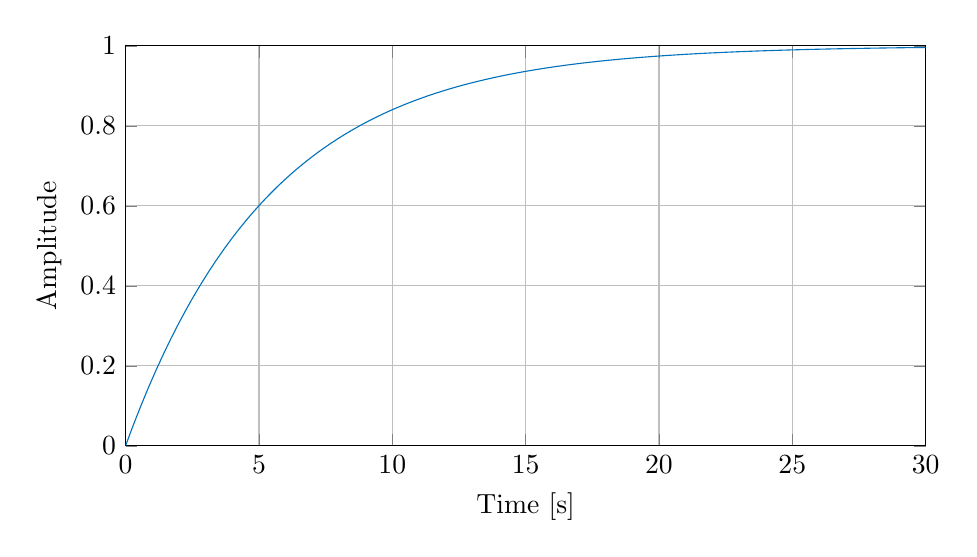
\begin{tikzpicture}

\begin{axis}[%
width=4in,
height=2in,
at={(1.011in,0.642in)},
scale only axis,
xmin=0,
xmax=30,
xlabel={Time [s]},
xmajorgrids,
ymin=0,
ymax=1,
ylabel={Amplitude},
ymajorgrids,
axis background/.style={fill=white}
]
\addplot [color=mycolor1,solid,forget plot]
  table[row sep=crcr]{%
0	0.000518798828125\\
0.283018867924528	0.0510624403982904\\
0.566037735849057	0.0990500962228728\\
0.849056603773585	0.144611022187057\\
1.13207547169811	0.187867937721793\\
1.41509433962264	0.228937356351479\\
1.69811320754717	0.267929899525898\\
1.9811320754717	0.304950594581707\\
2.26415094339623	0.340099157636049\\
2.54716981132075	0.37347026217427\\
2.83018867924528	0.405153794055194\\
3.11320754716981	0.435235093620804\\
3.39622641509434	0.463795185562473\\
3.67924528301887	0.490910997162882\\
3.9622641509434	0.516655565501479\\
4.24528301886792	0.541098234181575\\
4.52830188679245	0.564304840108977\\
4.81132075471698	0.586337890825256\\
5.09433962264151	0.607256732873284\\
5.37735849056604	0.627117711648547\\
5.66037735849057	0.645974323166804\\
5.94339622641509	0.663877358156869\\
6.22641509433962	0.680875038866639\\
6.50943396226415	0.697013148950857\\
6.79245283018868	0.71233515679047\\
7.07547169811321	0.72688233257574\\
7.35849056603774	0.740693859468478\\
7.64150943396226	0.753806939142814\\
7.92452830188679	0.766256891988789\\
8.20754716981132	0.778077252248655\\
8.49056603773585	0.789299858342155\\
8.77358490566038	0.799954938624056\\
9.05660377358491	0.810071192804937\\
9.33962264150943	0.81967586925454\\
9.62264150943396	0.828794838395894\\
9.90566037735849	0.837452662387916\\
10.188679245283	0.84567266128416\\
10.4716981132075	0.853476975845941\\
10.7547169811321	0.860886627178988\\
11.0377358490566	0.867921573354302\\
11.3207547169811	0.874600763165681\\
11.6037735849057	0.880942187168749\\
11.8867924528302	0.886962926138942\\
12.1698113207547	0.89267919707898\\
12.4528301886792	0.898106396899749\\
12.7358490566038	0.903259143892241\\
13.0188679245283	0.908151317102271\\
13.3018867924528	0.912796093714009\\
13.5849056603774	0.917205984543041\\
13.8679245283019	0.921392867734546\\
14.1509433962264	0.925368020757359\\
14.4339622641509	0.929142150780104\\
14.7169811320755	0.932725423511201\\
15	0.936127490580444\\
15.2830188679245	0.939357515535895\\
15.5660377358491	0.942424198526115\\
15.8490566037736	0.945335799734221\\
16.1320754716981	0.948100161626885\\
16.4150943396226	0.950724730078202\\
16.6981132075472	0.95321657442533\\
16.9811320754717	0.955582406509913\\
17.2641509433962	0.957828598756591\\
17.5471698113208	0.959961201337269\\
17.8301886792453	0.961985958467405\\
18.1132075471698	0.963908323878184\\
18.3962264150943	0.965733475506277\\
18.6792452830189	0.967466329440734\\
18.9622641509434	0.969111553164584\\
19.2452830188679	0.970673578126812\\
19.5283018867925	0.972156611678574\\
19.811320754717	0.973564648405795\\
20.0943396226415	0.97490148088868\\
20.377358490566	0.976170709917117\\
20.6603773584906	0.977375754189494\\
20.9433962264151	0.978519859521041\\
21.2264150943396	0.97960610758651\\
21.5094339622642	0.980637424220739\\
21.7924528301887	0.981616587299459\\
22.0754716981132	0.982546234221566\\
22.3584905660377	0.983428869013016\\
22.6415094339623	0.984266869071482\\
22.9245283018868	0.985062491569929\\
23.2075471698113	0.985817879536361\\
23.4905660377358	0.986535067626121\\
23.7735849056604	0.987215987602279\\
24.0566037735849	0.987862473538884\\
24.3396226415094	0.988476266761088\\
24.622641509434	0.989059020535442\\
24.9056603773585	0.989612304523009\\
25.188679245283	0.990137609007289\\
25.4716981132075	0.990636348908325\\
25.7547169811321	0.99110986759383\\
26.0377358490566	0.991559440497575\\
26.3207547169811	0.991986278554801\\
26.6037735849057	0.992391531463905\\
26.8867924528302	0.992776290783175\\
27.1698113207547	0.993141592870931\\
27.4528301886792	0.993488421676983\\
27.7358490566038	0.993817711392916\\
28.0188679245283	0.994130348968363\\
28.3018867924528	0.994427176500024\\
28.5849056603774	0.99470899349987\\
28.8679245283019	0.994976559048651\\
29.1509433962264	0.995230593840496\\
29.4339622641509	0.995471782124124\\
29.7169811320755	0.995700773545874\\
30	0.995749576707511\\
};
\end{axis}
\end{tikzpicture}%
	\caption{Step response.}
	\label{fig:releaseTimeDigitalStep}
\end{subfigure}
\caption{Frequency response and step response of the quantized digital filter. The sampling rate for the filter in this example is $f_s = 375$ Hz.}
\label{fig:releaseTime}
\end{figure}

In it is seen in \autoref{fig:releaseTime} that the frequency response and step response remains intact after quantization.

\subsection*{Implementation of Release Time}

To implement the release time, the transfer function from \autoref{eq:releaseTF} is first reduced:
\begin{equation}
H(z) = \frac{0.2T}{1-\text{e}^{-0.2T} z^{-1}}  \Leftrightarrow (1-\text{e}^{-0.2T} z^{-1})Y(z) = (0.2T)X(z) \Rightarrow Y(z) = 0.2TX(z) + \text{e}^{-0.2T} z^{-1}Y(z)
\end{equation}
Applying the inverse z-transformation (See \autoref{ch:IIR} for in debt explanation) reveals:
\begin{align}
y[n] = 0.2Tx[n] + {\rm e}^{- 0.2\,T}y[n-1]
\label{eq:z_eq}
\end{align}

The b-coefficients and a-coefficients from \autoref{eq:z_eq} be found as:
\begin{align}
b_{\text{IIR}} &= 0.2T \\
a_{\text{IIR}} &= {\rm e}^{- 0.2\,T}
\label{eq:Coef}
\end{align}

As IIR filter have a feedback loop, noise will be added because of the quantized output. To avoid this, double precision or noise shaping can be applied to overcome this problem. Since the accumulators are 40-bits, implementing a double precision algorithm requires splitting the IIR calculation up into two. Therefore noise shaping is used as it is simpler implement. Noise shaping works by feeding the lowest 16-bit of the output y[n] back into the next filter calculation before the quantization. The filter structure with noise shaping is shown in \autoref{fig:IIRFilterReleaseTime}. The coefficient can now be calculated by \autoref{eq:Coef} and then implemented using \autoref{eq:z_eq}. The coefficient are before implementation rewritten into Q15 format.

\begin{figure}[H]
\centering
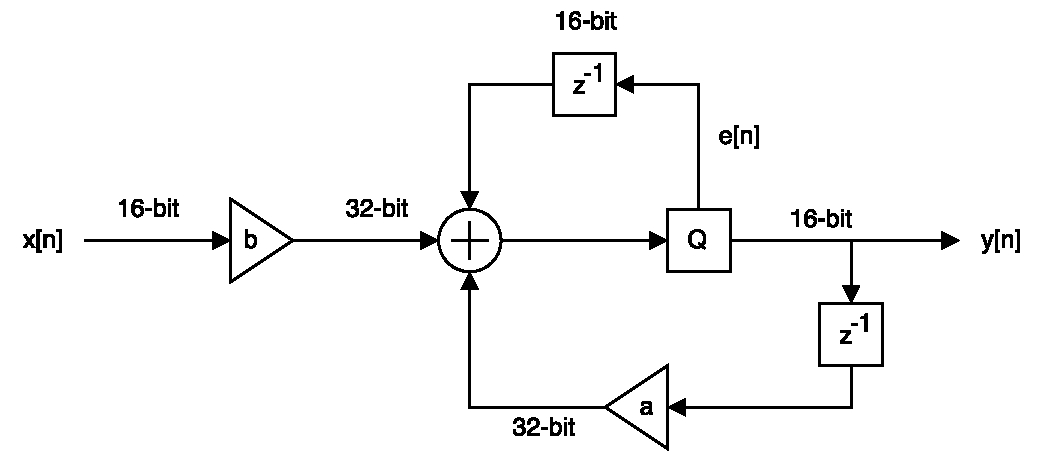
\includegraphics[width=0.7\textwidth]{IIRFilterReleaseTime}
\caption{Filter structure of IIR filter for release.}
\label{fig:IIRFilterReleaseTime}
\end{figure}

The IIR filter is implemented in assembly and is seen in \autoref{listingCompressorMain}. 

\begin{lstlisting}[language={[x86masm]Assembler}, caption = {Release time algorithm.},label={listingCompressorMain}]
_IIRFilter
	MOV #0, AC3				; Clear AC3
	MOV *(#OutPrev), T1		; Load T1 with the previous calculated RMS gain
	ADD *(#ErrorQ), AC3		; Add the quantized bits from the previous calculation (Noise shaping)
	MACM *(#bIIR),AC0,AC3	; Multiply and accumulate b coef and RMS gain from LUT
	MACM *(#aIIR),T1,AC3	; Multiply and accumulate a coef and Previous filtered RMS gain
	MOV AC3, *(#ErrorQ)		; Save lowest 16-bit as the quantation noise
	
	MOV *(#prevGain), T2
	MOV HI(AC0),T3
	CMP T3==T2, TC1
	CALLCC checkGain, !TC1
	
	SFTL AC3, #-15
	MOV AC3, *(#OutPrev)
	MOV AC3, *(#prevGain)
	RET

releaseOn:
	MOV AC3,AC0
	SFTL AC0, #-15
	SFTL AC0, #16
	RET
	

checkGain:
	MAX T3, T2				; if previous gain (T2) is less(RMS was bigger) than new gain (high bits of AC0), set CARRY = 1
	CMP T3==T2, TC1
	CALLCC releaseOn, TC1
	RET
\end{lstlisting}

The filter is executed when the routine for the RMS limiter is called. The filter is only applied when ever the previous output is lower than the current. This is to only apply the filter on the release and not attack.




